\hypertarget{persistencia}{%
\section{Persistence}\label{persistencia}}

\index{persistencia} \index{memoria secundaria}

So far, we have learned how to write programs and communicate our intentions to the \emph{Central Processing Unit} using conditional executions, functions and iterations. We have learned how to create and use data structures in \emph{Main Memory}. The CPU and memory are the places where our software works and runs. It's where all the \emph{intelligence} happens.

But if you remember our hardware architecture discussions, once the power goes out, anything stored either in the CPU or in memory is deleted. So until now our programs have been just a passing fun to learn Python. 

\begin{figure}
\centering

\includegraphics[width=0.5\textwidth]{images/sm.jpg}
\caption{Secondary Memory}
\end{figure}

In this chapter, we are going to start working with \emph{Secondary Memory} (or files). Secondary memory is not deleted when we turn off a computer. Even in the case of a USB memory, the data that we write from our programs can be removed from the system and transported to another system.

We are going to focus mainly on reading and writing files like the ones we create in a text editor. Later we will see how to work with database files, which are binary files specifically designed to be read and written by database management software.

\hypertarget{abrir-ficheros}{%
\section{Opening files}\label{abrir-ficheros}}

\index{fichero!abrir} \index{abrir función} \index{función!abrir}

When we want to open or write a file (for example, to the hard drive), we must first \emph{open} the file. When opening the file we communicate with the operating system, which knows where the data of each file is stored. When you open a file, you are asking the operating system to find the file by name and make sure it exists. In this example, we open the file \emph{mbox.txt}, which should be stored in the same directory you are located in when you start Python. You can download this file in Poliformat.

\begin{Verbatim}[frame=single][frame=single]
>>> file_handler = open('mbox.txt')
>>> print(file_handler)
  <_io.TextIOWrapper name='mbox.txt' mode='r' encoding='cp1252'>
\end{Verbatim}

\index{manejador fichero}

If the \pythoninline{open} is successful, the operating system returns a \emph{file handler}. The file handler is not the data contained in the file, but a handler that we can use to read the data. You will get a file handler if the requested file exists and if you have the appropriate permissions to read it.

\begin{figure}
\centering
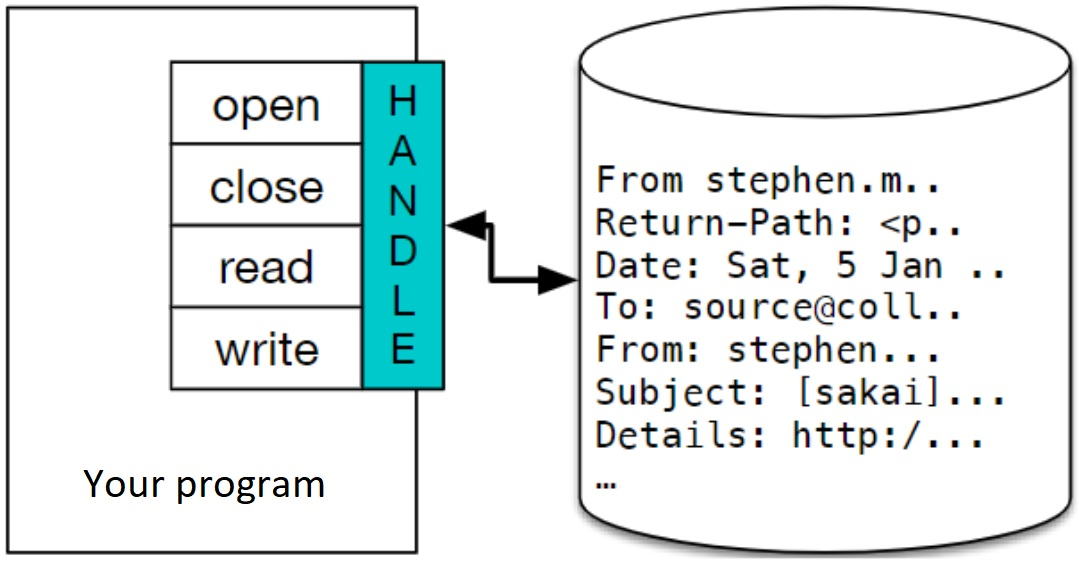
\includegraphics[width=0.6\textwidth]{images/ha.jpg}
\caption{A file handler}
\end{figure}

If the file doesn't exist, \pythoninline{open} will fail with an error message and you won't get a handler to access the contents of the file:

\begin{Verbatim}[frame=single][frame=single]
>>> file_handler = open('stuff.txt')
Traceback (most recent call last):
File "<stdin>", line 1, in <module>
FileNotFoundError: [Errno 2] No such file or directory: 'stuff.txt'
\end{Verbatim}

Later we will use \pythoninline{try} and \pythoninline{except} to better handle the situation where we try to open a file that doesn't exist.

\hypertarget{ficheros-de-texto-y-luxedneas}{%
\section{Text files and lines}\label{ficheros-de-texto-y-luxedneas}}

A text file can be thought of as a sequence of lines, just as a Python string can be thought of as a sequence of characters. For example, here is an example of a text file that records the email activity of some people on a development team in an open source project:

\begin{Verbatim}[frame=single]
From stephen.marquard@uct.ac.za Sat Jan  5 09:14:16 2008
Return-Path: <postmaster@collab.sakaiproject.org>
Date: Sat, 5 Jan 2008 09:12:18 -0500
To: source@collab.sakaiproject.org
From: stephen.marquard@uct.ac.za
Subject: [sakai] svn commit: r39772 - content/branches/
Details: http://source.sakaiproject.org/viewsvn/?view=rev&rev=39772
...
\end{Verbatim}

The complete file of email interactions is available in Poliformat under the name \texttt{mbox.txt} and a shortened version of the file is available in \texttt{mbox-short.txt}.

Those files are in a standard format for a file containing multiple mail messages. Lines beginning with ``From'' separate messages, and lines beginning with ``From:'' are part of those messages. For more information about the mbox format, see \url{https://en.wikipedia.org/wiki/Mbox}.

To separate the file into lines, there is a special character that represents the ``end of a line'' called \emph{line break}.

\index{saltodelinea}

In Python, we represent the \emph{line break} as a backslash+n in strings. Even though this looks like two characters, it really is a single character. When we see the variable interacting with the interpreter, it shows us the \verb|\n| in the string, but when we use \pythoninline{print} to print the string, we see the string split across two lines due to the line break.

\begin{Verbatim}[frame=single][frame=single]
>>> thing = 'Hello\nWorld!'
>>> thing
'Hello\nWorld!'
>>> print(thing)
Hello
World!
>>> thing = 'X\nY'
>>> print(thing)
X
Y
>>> len(thing)
3
\end{Verbatim}

You can also see that the size of the string \verb|X\nY| is \emph{three} characters because the line separator is a single character.

Therefore, when we see the lines in a file, we need to \emph{imagine} that there is an invisible character called a line separator at the end of each line, which marks the end of the line.

So the line separator separates the characters in the file into lines.

\hypertarget{lectura-de-ficheros}{%
\section{Reading files}\label{lectura-de-ficheros}}

\index{fichero!lectura} \index{contador}

Although the \emph{file handler} does not contain the data of a file, it is quite easy to use it in a \pythoninline{for-in} loop to read through the file and count each of its lines:

\begin{python}[frame=single]
file_handler = open('mbox-short.txt')
counter = 0
for line in file_handler:
    counter = counter + 1
print('Line counter:', counter)
\end{python}

We can use the file handler as a sequence in our \pythoninline{for} loop. Our \pythoninline{for} loop simply counts the number of lines in the file and prints them. The rough translation of that loop is, ``for each line in the file represented by the file handler, add one to the \pythoninline{count} variable.''

The reason the \pythoninline{open} function doesn't read the entire file is because the file can be very large, even with many gigabytes of data. The \pythoninline{open} statement takes the same amount of time regardless of the size of the file. In fact, it is the \pythoninline{for} loop that causes the data to be read from the file.

When the file is read using a \pythoninline{for} loop in this way, Python takes care of splitting the data in the file onto separate lines using the line separator. Python reads each line up to the separator and includes the separator as the last character in the variable \pythoninline{line} for each iteration of the \pythoninline{for} loop.

Because the \pythoninline{for} loop reads data line by line, it can efficiently read and count lines in very large files without running out of main memory to store the data. The previous program can count the lines of any file size using little memory, since each line is read, counted, and then discarded.

If you know that the file is relatively small compared to the size of your main memory, you can read the entire file in a single string using the \pythoninline{read} method on the file handler.

\begin{Verbatim}[frame=single][frame=single]
>>> file_handler = open('mbox-short.txt')
>>> inp = file_handler.read()
>>> print(len(inp))
94626
>>> print(inp[:20])
From stephen.marquar
\end{Verbatim}

In this example, the full content (all 94626 characters) of the file \emph{mbox-short.txt} are read directly into the variable \pythoninline{inp}. We use string slicing to print the first 20 characters of the data string stored in \pythoninline{inp}.

When the file is read this way, all characters including line breaks are one giant string in the \pythoninline{inp} variable. It's a good idea to store the output of \pythoninline{read} as a variable because each call to \pythoninline{read} empties the content completely:

\begin{Verbatim}[frame=single][frame=single]
>>> handler = open('mbox-short.txt')
>>> print(len(handler.read()))
94626
>>> print(len(handler.read()))
0
\end{Verbatim}

Remember that this form of the \pythoninline{open} function should only be used if the data in the file is appropriate for the system's main memory. If the file is too large to fit in main memory, you should write your program to read the file in blocks using a \pythoninline{for} or \pythoninline{while} loop.

\hypertarget{buxfasqueda-a-travuxe9s-de-un-fichero}{%
\section{Searching through a file}\label{buxfasqueda-a-travuxe9s-de-un-fichero}}

When searching through the data in a file, a very common pattern is to read the file, ignore most of the lines, and only process lines that meet a particular condition. We can combine the pattern of reading a file with string methods to build simple search mechanisms.

\index{filtro patron} \index{patron!filtro}

For example, if we wanted to read a file and only print the lines that start with the ``From:'' prefix, we could use the \emph{startswith} string method to select only those lines with the desired prefix:

%%\VerbatimInput{../code3/search1.py}
\begin{python}[frame=single]
man_f = open('mbox-short.txt')
counter = 0
for line in man_f:
    if line.startswith('From:'):
        print(line)
\end{python}

When this program runs, we get the following output:

\begin{Verbatim}[frame=single]
From: stephen.marquard@uct.ac.za

From: louis@media.berkeley.edu

From: zqian@umich.edu

From: rjlowe@iupui.edu
...
\end{Verbatim}

The output looks correct since the lines we're looking for are those that start with ``From:'', but why are we seeing the extra empty lines? This is due to the invisible \emph{newline} character. Each line read ends with a newline, so the \pythoninline{print} statement prints the string stored in the variable \pythoninline{line}, which includes that newline, and then \pythoninline{print} adds \emph{another} newline, resulting in the double-newline effect we see.

We can use line striping to print all but the last character, but an easier way is to use the \pythoninline{rstrip} method, which strips whitespace from the right side of a string, like so:

%\VerbatimInput{../code3/search2.py}
\begin{python}[frame=single]
man_f = open('mbox-short.txt')
for line in man_f:
    line = line.rstrip()
    if line.startswith('From:'):
        print(line)
\end{python}

When this program runs, we get the following:

\begin{Verbatim}[frame=single]
From: stephen.marquard@uct.ac.za
From: louis@media.berkeley.edu
From: zqian@umich.edu
From: rjlowe@iupui.edu
From: zqian@umich.edu
From: rjlowe@iupui.edu
From: cwen@iupui.edu
...
\end{Verbatim}

As your file processing programs get more complicated, you may want to structure your search loops using \pythoninline{continue}. The basic idea of a search loop is that you are looking for ``interesting'' lines and ignoring ``uninteresting'' lines. And when we find an interesting line, we do something with it.

We can structure the loop to follow the pattern of ignoring uninteresting lines like this:

%\VerbatimInput{../code3/search3.py}
\begin{python}[frame=single]
man_f = open('mbox-short.txt')
for line in man_f:
    line = line.rstrip()
    # Ignore lines we are not interested in
    if not line.startswith('From:'):
        continue
    # Process the line we are interested in
    print(line)

\end{python}

The output of the program is the same. The uninteresting lines are those that don't start with ``From:'', so we skip them using \pythoninline{continue}. Instead the ``interesting'' lines (those starting with ``From:'') are processed.

We can use the \pythoninline{find} string method to simulate a text editor's find function, which finds lines where the search string appears somewhere. Since \pythoninline{find} looks for any occurrence of a string within another string and returns the position of that string or -1 if the string was not found, we can write the following loop to display lines containing the string ``@uct.ac.za'' (i.e. those coming from the University of Cape Town in South Africa):

%\VerbatimInput{../code3/search4.py}
\begin{python}[frame=single]
man_f = open('mbox-short.txt')
for line in man_f:
    line = line.rstrip()
    if line.find('@uct.ac.za') == -1: continue
    print(line)
\end{python}

Which produces the following output:

\begin{Verbatim}[frame=single]
From stephen.marquard@uct.ac.za Sat Jan  5 09:14:16 2008
X-Authentication-Warning: set sender to stephen.marquard@uct.ac.za using -f
From: stephen.marquard@uct.ac.za
Author: stephen.marquard@uct.ac.za
From david.horwitz@uct.ac.za Fri Jan  4 07:02:32 2008
X-Authentication-Warning: set sender to david.horwitz@uct.ac.za using -f
From: david.horwitz@uct.ac.za
Author: david.horwitz@uct.ac.za
...
\end{Verbatim}

Here we use the contracted form of the \pythoninline{if} statement where we put the \pythoninline{continue} on the same line as the \pythoninline{if}. This collapsed form of the \pythoninline{if} works the same way as if the \pythoninline{continue} were on the next line and indented.

\hypertarget{permitiendo-al-usuario-elegir-el-nombre-de-fichero}{%
\section{Allowing the user to choose the filename}\label{permitiendo-al-usuario-elegir-el-nombre-de-fichero}}

We definitely don't want to have to edit our Python code every time we want to process a different file. It would be more useful to ask the user to enter the filename each time the program runs, so that you can use our program on different files without having to change the code.

This is easy to do by reading the user's filename using \pythoninline{input} as shown below:

%\VerbatimInput{../code3/search6.py}
\begin{python}[frame=single]
name_f = input('Enter a filename: ')
man_f = open(name_f)
counter = 0
for line in man_f:
    if line.startswith('Subject:'):
        counter = counter + 1
print('There are ', counter, ' subject lines in ', name_f)
\end{python}

We read the user's filename and we store it in a variable called \pythoninline{man_f}. Then we open the file. Now we can run the program repeatedly on different files.

\begin{Verbatim}[frame=single]
>>> %Run
  Enter a filename: mbox.txt
  There are 1797 subject lines in mbox.txt
>>> %Run
  Enter a filename: mbox-short.txt
  There are 27 subject lines in mbox-short.txt
\end{Verbatim}

Before looking at the next section, take a look at the above program and ask yourself, ``What error could I get here?'' or ``What could our friendly user do that would cause our little program to terminate unsuccessfully with an error, making us look not-so-cool in the eyes of our users?''

\hypertarget{utilizando-try-except-y-open}{%
\section{\texorpdfstring{Using try, except, and
open}{Using try, except, and open}}\label{utilizando-try-except-y-open}}

I told you not to look. This is your last chance.

What if our user types something that is not a filename?

\begin{Verbatim}[frame=single]
>>> %Run
Enter a filename: missing.txt
Traceback (most recent call last):
  File "search6.py", line 2, in <module>
    man_a = open(nfile)
FileNotFoundError: [Errno 2] No such file or directory: 'missing.txt'
>>> %Run
Enter a filename: na na boo boo
Traceback (most recent call last):
  File "search6.py", line 2, in <module>
    man_a = open(nfile)
FileNotFoundError: [Errno 2] No such file or directory: 'na na boo boo'
\end{Verbatim}

Do not laugh. Users will eventually do anything they can to break your programs, whether on purpose or without malicious intent. In fact, an important part of any software development team is a person or group called \emph{Quality Assurance} (or QA) whose job it is to try the craziest things possible in an attempt to make fail the software that the programmer has created.

\index{Control de Calidad} \index{QA}

The QA (Quality Control) team is responsible for finding bugs in programs before they are delivered to end users, who might buy our software or pay our salary to write it. So the QA team is a programmer's best friend.

\index{try sentencia} \index{sentencia!try} \index{abrir funcion}
\index{funcion!abrir} \index{excepcion!IOError} \index{IOError}

Now that we see the flaw in the program, we can fix it elegantly using the \pythoninline{try}/\pythoninline{except} structure. We need to assume that the \pythoninline{open} call might fail and add recovery code for that failure, like this:

%\VerbatimInput{../code3/search7.py}
\begin{python}[frame=single]
name_f = input('Enter a filename: ')
try:
    man_f = open(name_f)
except:
    print('Can't open file:', name_f)
    exit()
counter = 0
for line in man_f:
    if line.startswith('Subject:'):
        counter = counter + 1
print('There are ', counter, ' subject lines in ', name_f)
\end{python}

The \pythoninline{exit} function ends the program. It's a function we call that never returns anything. Now when our user (or the QA team) enters something nonsense or a wrong filename, we're going to ``catch'' it and gracefully recover:

\begin{Verbatim}[frame=single]
>>> %Run
Enter a filename: mbox.txt
There are 1797 subject lines in mbox.txt
>>> %Run
Enter a filename: na na boo boo
Can't open file: na na boo boo
\end{Verbatim}

\index{Pythonic}
Protecting the \pythoninline{open} call is a good example of the correct use of \pythoninline{try} and \pythoninline{except} in a Python program. We use the term ``pythonic'' when we are doing something ``Python style''. We could say that the previous example is a pythonic way of opening a file.

Once you're more familiar with Python, you can brainstorm with other Python programmers to decide which of two equivalent solutions to a problem is ``more pythonic''. The goal of being ``more pythonic'' encompasses the notion that programming is part engineering and part art. We are not always interested in just making something work, we also want our solution to be elegant and to be appreciated as elegant by our peers.

\hypertarget{escritura-de-ficheros}{%
\section{Writing files}\label{escritura-de-ficheros}}

\index{fichero!escritura}

To write to a file, you have to open it in ``w'' mode (for \pythoninline{write}) as the second parameter:

\begin{Verbatim}[frame=single][frame=single]
>>> fout = open('output.txt', 'w')
>>> print(fout)
<_io.TextIOWrapper name='output.txt' mode='w' encoding='cp1252'>
\end{Verbatim}

If the file already existed, opening it in write mode will cause the entire contents of the file to be deleted, so be careful! If the file does not exist, a new file is created.

The file handler's \pythoninline{write} method writes data into the file, returning the number of characters written. The default writing mode is text for writing (and reading) strings.

\begin{Verbatim}[frame=single][frame=single]
>>> line1 = "Here is the wattle,\n"
>>> fout.write(line1)
20
\end{Verbatim}

\index{saltodelinea}

The file handler keeps track of where it is, so if you call \pythoninline{write} again, it adds the new data to the end.

We must make sure to handle the endings of the lines as we write to the file, explicitly inserting the line break character when we want to end a line. The \pythoninline{print} statement adds a newline automatically, but the \pythoninline{write} method does not add one automatically.

\begin{Verbatim}[frame=single][frame=single]
>>> line2 = 'the symbol of our land.\n'
>>> fout.write(line2)
30
\end{Verbatim}

When you finish writing, you have to close the file to make sure that the last part of the data is physically written to the hard drive, so that the data is not lost if the power goes out.

\begin{Verbatim}[frame=single][frame=single]
>>> fsal.close()
\end{Verbatim}

We could close open files for reading as well, but we can be less rigorous if we're only opening a few files since Python makes sure that all open files are closed when the program ends. On the other hand, when we are writing files we must explicitly close them so as not to leave anything to chance.

\index{cerrar metodo} \index{metodo!cerrar}

\hypertarget{depuraciuxf3n}{%
\section{Debugging}\label{depuraciuxf3n}}

\index{depuracion} \index{espacioenblanco}

When you are reading and writing files, you may have problems with white space. Those errors can be difficult to debug because spaces, tabs and line breaks are normally invisible:

\begin{Verbatim}[frame=single]
>>> s = '1 2\t 3\n 4'
>>> print(s)
1 2  3
 4
\end{Verbatim}

\index{repr funcion} \index{funcion!repr} \index{cadena representacion}

The native function \pythoninline{repr} can help you. Takes any object as an argument and returns a representation of the object as a string. For strings, represent white space with backslash sequences:

\begin{Verbatim}[frame=single]
>>> print(repr(s))
'1 2\t 3\n 4'
\end{Verbatim}

This can be useful for debugging.

Another problem you might have is that different systems use different characters to indicate the end of a line. Some systems use a newline, represented as \textbackslash{}n. Others use a return character, represented by \textbackslash{}r. Others use both. If you move files between different systems, those inconsistencies could cause you problems.

\index{carácter final de linea}

For most systems, there are applications that convert from one format to another. You can find them (and read more about them) at \url{wikipedia.org/wiki/Newline}. Or, of course, you can also write one yourself.

\hypertarget{glosario}{%
\section{Glossary}\label{glosario}}

\begin{description}
\tightlist
\item[catch]
Prevent an exception from terminating a program, using the \pythoninline{try} and \pythoninline{except} statements.
\index{catch}

\item[line break]
A special character used in files and strings to indicate the end of a line.
\index{salto de línea}

\item[pythonic]
A technique that works elegantly in Python. ``Using try and except is the \emph{Pythonic} way of handling nonexistent files''.
\index{Pythonic}

\item[Quality Assurance (QA)]
A person or team focused on ensuring the overall quality of a product. Quality Assurance (QA) is often tasked with testing software and finding possible problems before the software is released.
\index{Control de calidad} \index{QA}

\item[textfile]
A sequence of characters stored on a permanent storage device such as a hard drive.
\index{fichero de texto}
\end{description}


\section*{Exercises}\label{ejercicios}
\addcontentsline{toc}{section}{Exercises}

\begin{exercise}
Write a program that reads the file \texttt{mbox-short.txt} and prints its contents (line by line), all in upper case. To test the program, run it and verify that this comes out:

\begin{Verbatim}[frame=single]
>>> %Run 
Enter a filename: mbox-short.txt
FROM STEPHEN.MARQUARD@UCT.AC.ZA SAT JAN  5 09:14:16 2008
RETURN-PATH: <POSTMASTER@COLLAB.SAKAIPROJECT.ORG>
RECEIVED: FROM MURDER (MAIL.UMICH.EDU [141.211.14.90])
     BY FRANKENSTEIN.MAIL.UMICH.EDU (CYRUS V2.3.8) WITH LMTPA;
     SAT, 05 JAN 2008 09:14:16 -0500
\end{Verbatim}

You can download the file \texttt{mbox-short.txt} from Poliformat.
\end{exercise}

\begin{exercise}
Write a program that asks for a file name and then reads that file looking for lines that have the following form:

\begin{Verbatim}[frame=single]
X-DSPAM-Confidence: 0.8475
\end{Verbatim}

**When you find a line that starts with ``X-DSPAM-Confidence:'' set it aside to extract the decimal number from the line. It counts those lines and then computes the running total of the ``spam-confidence'' values. When you get to the end of the file, print the average value of ``spam confidence''.

\begin{Verbatim}[frame=single]
>>> %Run
Enter a filename: mbox.txt
Average spam confidence: 0.894128046745

>>> %Run
Enter a filename: mbox-short.txt
Average spam confidence: 0.750718518519
\end{Verbatim}

Test your program with the files \texttt{mbox.txt} and
\texttt{mbox-short.txt} that are in Poliformat.
\end{exercise}


\begin{exercise}
Sometimes when programmers get bored or want to have a little fun, they add a harmless \emph{Easter Egg} to their program. Modify the program that asks the user for the filename so that it prints a funny message when the user types ``na na boo boo'' for the filename. The program should work normally for any file that exists or doesn't exist. Here are three examples to test your program:

\begin{Verbatim}[frame=single]
>>> %Run 
Enter a filename: mbox.txt
There are 1797 subject lines in mbox.txt

>>> %Run 
Enter a filename: inexistente.tyxt
Can't open file: inexistente.tyxt

>>> %Run 
Enter a filename: na na boo boo
NA NA BOO BOO PARA TI - I've got you!
\end{Verbatim}

We're not advising you to put Easter Eggs in your programs; it's just an exercise.
\end{exercise}



\begin{exercise}
Write a program that reads the name of a text file from the keyboard and displays the encoded text on the screen so that only the lowercase letters are replaced by the following.

For example, if the file is:

\begin{Verbatim}[frame=single, label={\em message.txt}]
This is a secret message
\end{Verbatim}


\begin{Verbatim}[frame=single]
>>> %Run 
Enter a filename: message.txt
Tijt jt b tfdsfu nfttbhf
\end{Verbatim}

Run tests for your function by creating different text files as input to your program and verify that the result is the expected output.



\end{exercise}


\begin{exercise}
We need to anonymize the file \texttt{interview.txt} in Poliformat. This file contains an interview with Bill, but his name cannot appear and must be changed to Charlie to anonymize the file. Your function has to return the name of the anonymized file.


Write a \pythoninline{anonymize} function in Python that can anonymize this file. The function receives 3 parameters, the name of a file and two strings \texttt{s1} and \texttt{s2}. Throughout the file you have to change the occurrences of \texttt{s1} for \texttt{s2}.

You can test your function manually using the file \texttt{interview.txt}

\begin{Verbatim}[frame=single]
>>> interview_file = "interview.txt"
>>> new_file = anonymize(interview_file, "Bill", "Charlie")
>>> handle_new_file = open(new_file)
>>> for l in handle_new_file:
    print(l)
    
Charlie is a Syrian refugee. He arrived three days..
........
........
\end{Verbatim}
\end{exercise}


\begin{exercise}
To test the previous exercise automatically, we are going to write another function, \pythoninline{in_file}, that takes as an argument a filename and a string, and returns \pythoninline{True} if the string appears in the file and \pythoninline{False} if it does not.

The idea is to test that our \pythoninline{anonymize} function has successfully anonymized the file, for example like this:

\begin{python}
@pytest.mark.parametrize("testcase, in1, in2, in3",[
(1, "interview.txt", "Bill", "Charlie")
])              

def test_anonymize(testcase, in1, in2, in3):
    assert not (in_file(anonymize(in1, in2, in3),in2)),\
           "case {0}".format(testcase)
\end{python}

Create 2 more text files to anonymize. This way you will add 2 test cases.

\end{exercise}



\begin{exercise} 
Write a function that asks for an integer \pythoninline{n} between 1 and 20 and saves the division table for that number in a file named table-div-n.txt, where \pythoninline{n} is the number entered. The file format is based on the number of digits of the numbers. For example:

\begin{tabular}{p{3cm}p{3cm}p{3cm}}

\pythoninline{n} is 13:

\begin{verbatim}
 13 : 13 =  1
 26 : 13 =  2
 39 : 13 =  3
 52 : 13 =  4
 65 : 13 =  5
 78 : 13 =  6
 91 : 13 =  7
104 : 13 =  8
117 : 13 =  9
130 : 13 = 10
\end{verbatim}
&
\pythoninline{n} is 3:

\begin{verbatim}
  3 :  3 =  1
  6 :  3 =  2
  9 :  3 =  3
 12 :  3 =  4
 15 :  3 =  5
 18 :  3 =  6
 21 :  3 =  7
 24 :  3 =  8
 27 :  3 =  9
 30 :  3 = 10
\end{verbatim}

& 
\pythoninline{n} is 1:

\begin{verbatim}
  1 :  1 =  1
  2 :  1 =  2
  3 :  1 =  3
  4 :  1 =  4
  5 :  1 =  5
  6 :  1 =  6
  7 :  1 =  7
  8 :  1 =  8
  9 :  1 =  9
 10 :  1 = 10
\end{verbatim}
\end{tabular}

That is, the number of spaces can be a maximum of 8 in a line (as in the case of 1). Test your function by hand with some values.


\end{exercise}

\begin{exercise}
To make the testing of the previous exercise a little easier, and to avoid having to open and close files all the time, we are going to write a function \pythoninline{print_table} that asks for an integer $n$ between 1 and 10, read the table-div-n.txt file generated with the division table of that number and display it on the screen. If the file does not exist, a message should be displayed on the screen informing about it.
\end{exercise}


\begin{exercise}
In the end we decided to automate the testing of the function to make the testing of the previous exercise even easier, and to avoid having to open and close files all the time. Let's write a function \pythoninline{check_table} that asks for an integer $n$ between 1 and 10, reads the file table-div-n.txt generated with the division table of that number and returns \pythoninline{True} if the file is correct and \pythoninline{False} if not. If the file does not exist, a message should be displayed on the screen informing about it.


\begin{python}
@pytest.mark.parametrize("testcase, input",[
(1, 3),
(2, 5),
(4, 9),
(10, 11)
])              

def test_tabla_division(testcase, input):
    tabla_division(input)
    assert check_tabla(input),"case {0}".format(testcase)
\end{python}
\end{exercise}

\begin{exercise}
\label{generate_ficheros}
Write a function \pythoninline{generate_files} in Python that can generate a number of files with a random number (between 2 and 20) of random real numbers (between 1.00 and 300.00). The numbers have to be aligned to the right and with 3 decimal places.

%Puedes importar \pythoninline{random} y usar \pythoninline{randint} para generar números enteros de forma aleatorio, y \pythoninline{uniform} para generar números reales de forma aleatorio.

Your function receives 2 parameters:

\begin{itemize}
    \item the number of files you want to generate
    \item the name you want to use as the base of the generated files. For example, the quantity to generate is 4 files with base name\texttt{file}, your function will generate the files \texttt{file1.txt}, \texttt{file2.txt}, \dots, \texttt{file4.txt }
\end{itemize}

For example:

\begin{Verbatim}[frame=single, label={\em interactive session example}]
>>> generate_files(4, "file")
>>> 
\end{Verbatim}

It can generate for example:

\begin{tabular}{p{3cm}p{3cm}p{3cm}p{3cm}}

\begin{Verbatim}[frame=single, label={\em file1.txt}]
 133.252 
 159.931 
 162.024 
  23.260 
 147.501 
\end{Verbatim}
&
\begin{Verbatim}[frame=single, label={\em file2.txt}]
  29.921 
 199.442 
 158.016 
\end{Verbatim}
&
\begin{Verbatim}[frame=single, label={\em file3.txt}]
  50.082 
  59.349
 109.880
 153.481
 195.162
  51.953
  86.554
 153.281
\end{Verbatim}
&
\begin{Verbatim}[frame=single, label={\em file4.txt}]
   6.640
 136.339
  32.027
  56.166
  97.675
 160.564
\end{Verbatim}
\end{tabular}

\end{exercise}

\begin{exercise}
Write a function \pythoninline{file2list} that takes the name of a file and reads a number of real numbers from this file, storing them in a list. Your function has to return the list. 


\begin{Verbatim}[frame=single, label={\em interactive session example}]
>>> file2list("file2.txt")
[29.921 , 199.442 , 158.016]

>>>file2list("file4.txt")
>>>[6.640, 136.339, 32.027, 56.166, 97.675, 160.564]
\end{Verbatim}

\end{exercise}

\begin{exercise}
Write a function \pythoninline{calculate\_formula} in Python that receives the name of a file and that reads an amount ($N$) of real numbers from this file, stores them in a list $l$, and displays on the screen the value of applying a formula to such data.

The value of the formula is calculated as the sum of the squared differences between each element of the list, $l[i]$, and the \emph{mean}, all divided by the number of elements ($N$) :
\begin{equation}
  formula = \frac{\sum_{i=1}^{N} (x[i]-mean)^{2}}{N-1}
\end{equation}

%La media de una lista podemos obtener usando sum()/len().

For example, imagine we have:

\begin{Verbatim}[frame=single, label={\em numbers.txt}]
   6.64 
 136.33 
  32.02 
  56.16 
  97.67 
 160.56 
\end{Verbatim}


\begin{Verbatim}[frame=single, label={\em function call example}]
>>> calculate_formula("numbers.txt")
 3642.5325866666667
\end{Verbatim}

To test your solution you can use the following pytest:

\begin{python}
import pytest
import statistics

@pytest.mark.parametrize("testcase, f_input",[
(1,  "numbers1.txt"),
(2,  "numbers2.txt"),
(3,  "numbers3.txt"),
(4,  "numbers4.txt"),
])

def test_your_function(testcase, f_input):
    generate_files(4, "numbers")
    your_formula = calculate_formula(f_input)
    formula = statistics.variance(file2list(f_input))
    assert abs(your_formula - formula) < 10**-7 ,\
           "case {0} has failed".format(testcase)
\end{python}




\end{exercise}




